%!TeX root=../pridetop.tex
\chapter[Chapter \thechapter]{}
	
\begin{figure}[t!]
\centering
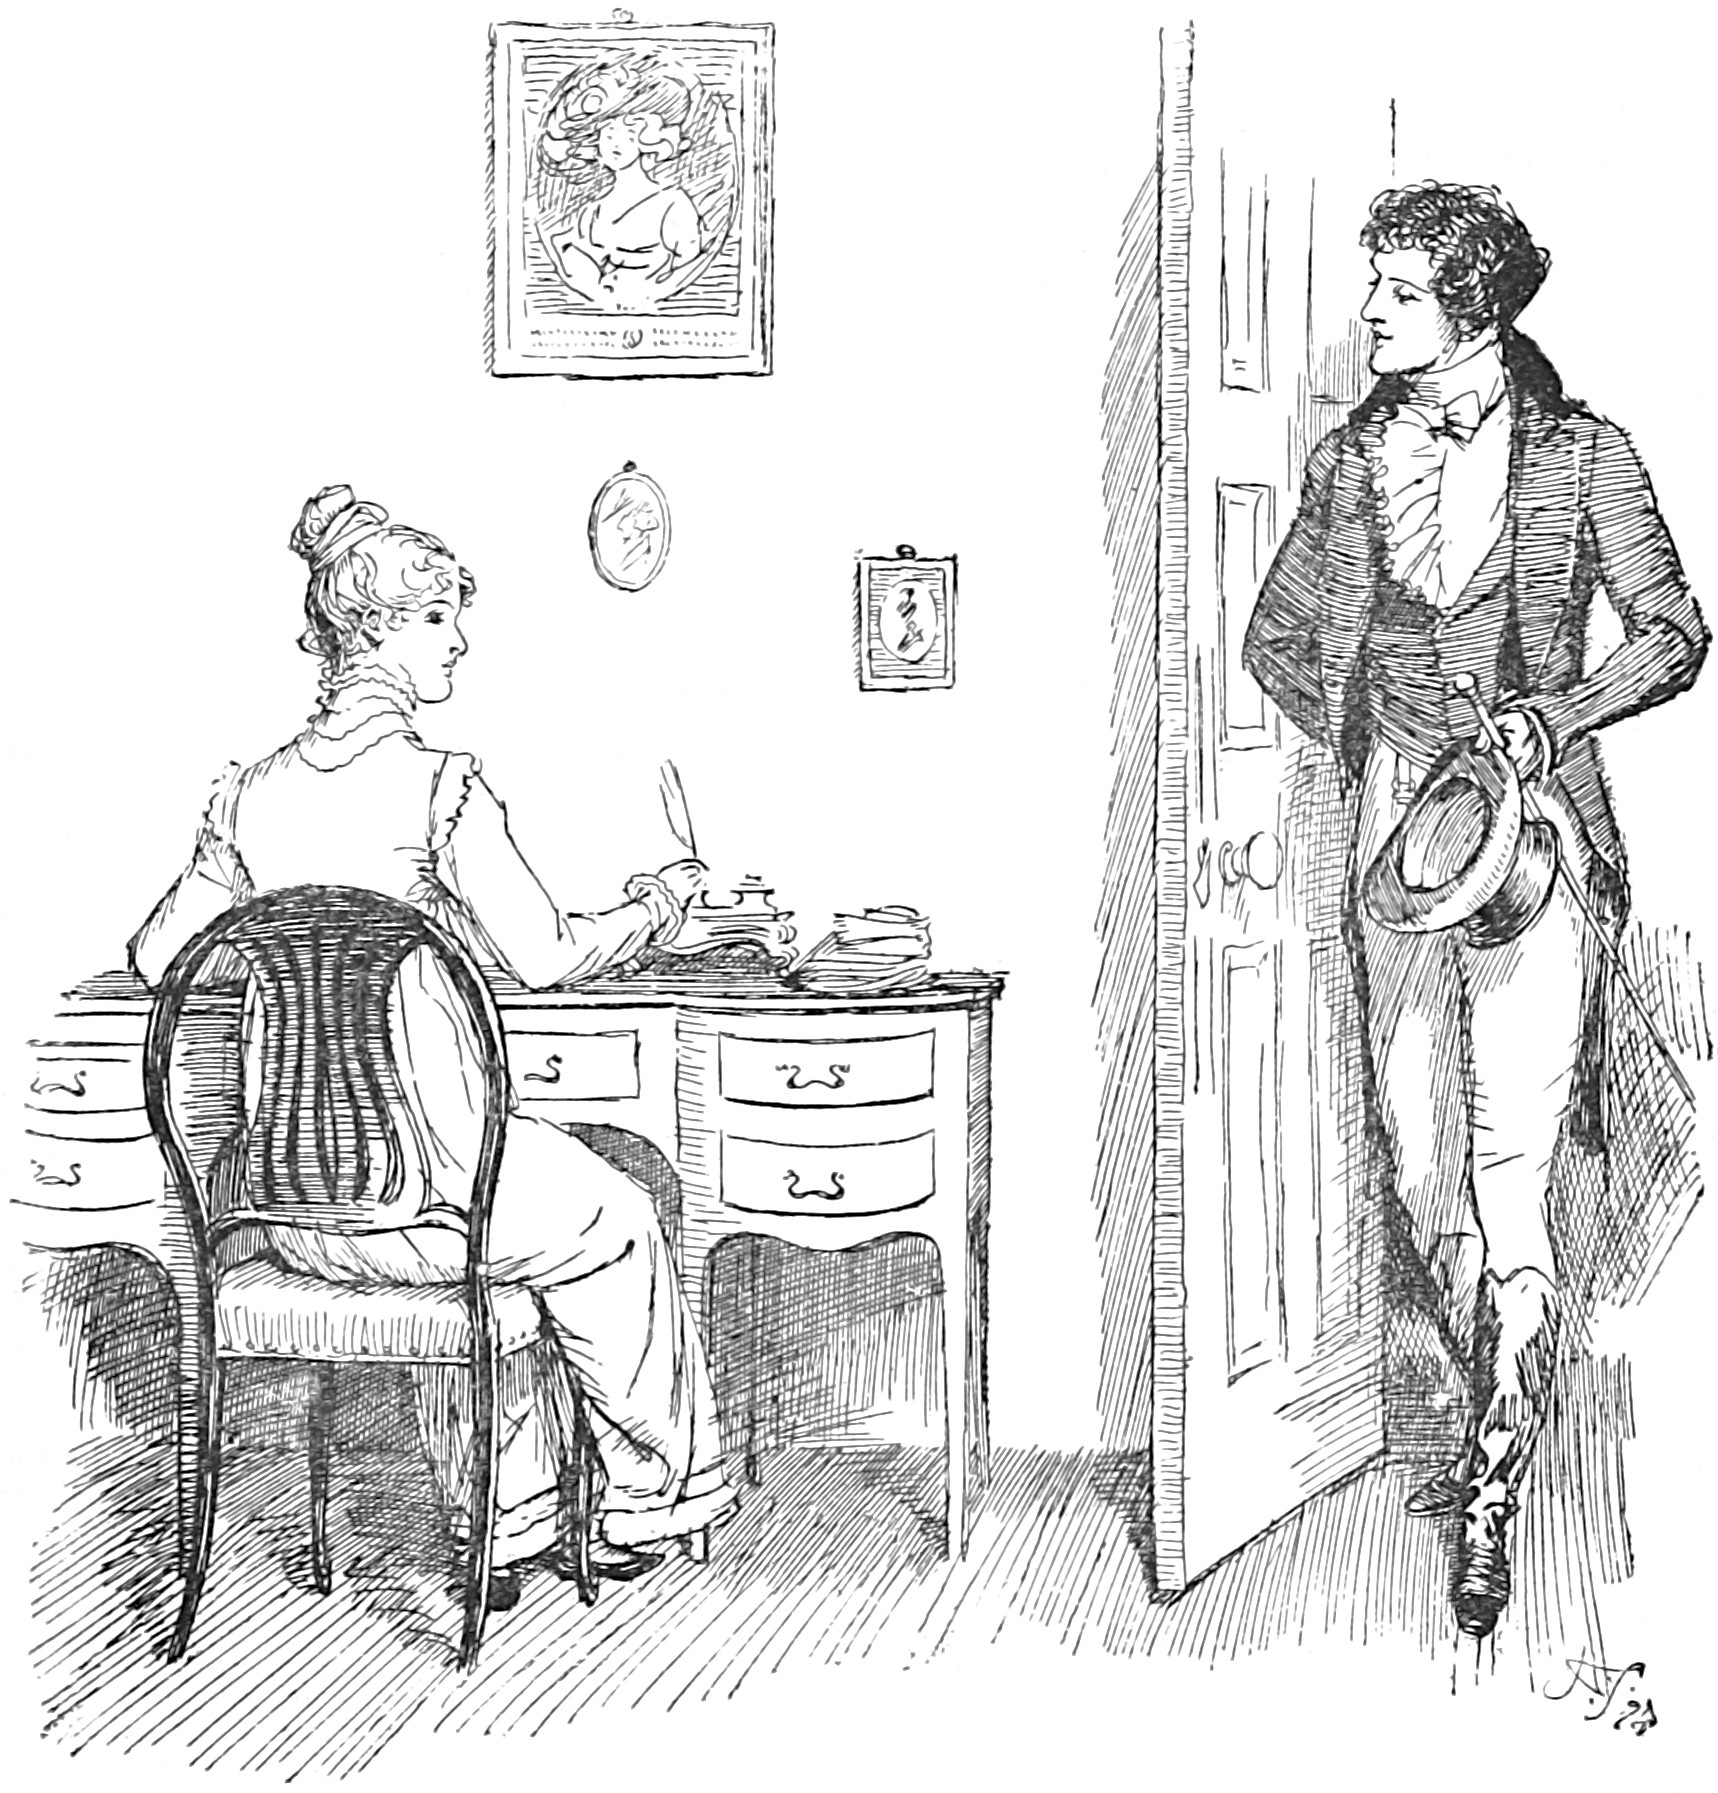
\includegraphics[width=.8\linewidth]{32top}
\captionlistentry{Headpiece to Chapter \thechapter}
\end{figure}


\lettrine[lines=6,image=true]{initials/chap32e}{lizabeth} was sitting by herself the next morning, and writing to Jane, while Mrs Collins and Maria were gone on business into the village, when she was startled by a ring at the door, the certain signal of a visitor. As she had heard no carriage, she thought it not unlikely to be Lady Catherine; and under that apprehension was putting away her half-finished letter, that she might escape all impertinent questions, when the door opened, and to her very great surprise Mr Darcy, and Mr Darcy only, entered the room.

He seemed astonished too on finding her alone, and apologized for his intrusion, by letting her know that he had understood all the ladies to be within.

They then sat down, and when her inquiries after Rosings were made, seemed in danger of sinking into total silence. It was absolutely necessary, therefore, to think of something; and in this emergency recollecting \textit{when} she had seen him last in Hertfordshire, and feeling curious to know what he would say on the subject of their hasty departure, she observed,—

»How very suddenly you all quitted Netherfield last November, Mr Darcy! It must have been a most agreeable surprise to Mr Bingley to see you all after him so soon; for, if I recollect right, he went but the day before. He and his sisters were well, I hope, when you left London?«

»Perfectly so, I thank you.«

She found that she was to receive no other answer; and, after a short pause, added,—

»I think I have understood that Mr Bingley has not much idea of ever returning to Netherfield again?«

»I have never heard him say so; but it is probable that he may spend very little of his time there in future. He has many friends, and he is at a time of life when friends and engagements are continually increasing.«

»If he means to be but little at Netherfield, it would be better for the neighbourhood that he should give up the place entirely, for then we might possibly get a settled family there. But, perhaps, Mr Bingley did not take the house so much for the convenience of the neighbourhood as for his own, and we must expect him to keep or quit it on the same principle.«

»I should not be surprised,« said Darcy, »if he were to give it up as soon as any eligible purchase offers.«

Elizabeth made no answer. She was afraid of talking longer of his friend; and, having nothing else to say, was now determined to leave the trouble of finding a subject to him.

He took the hint and soon began with, »This seems a very comfortable house. Lady Catherine, I believe, did a great deal to it when Mr Collins first came to Hunsford.«

»I believe she did—and I am sure she could not have bestowed her kindness on a more grateful object.«

»Mr Collins appears very fortunate in his choice of a wife.«

»Yes, indeed; his friends may well rejoice in his having met with one of the very few sensible women who would have accepted him, or have made him happy if they had. My friend has an excellent understanding—though I am not certain that I consider her marrying Mr Collins as the wisest thing she ever did. She seems perfectly happy, however; and, in a prudential light, it is certainly a very good match for her.«

»It must be very agreeable to her to be settled within so easy a distance of her own family and friends.«

»An easy distance do you call it? It is nearly fifty miles.«

»And what is fifty miles of good road? Little more than half a day's journey. Yes, I call it a very easy distance.«

»I should never have considered the distance as one of the \textit{advantages} of the match,« cried Elizabeth. »I should never have said Mrs Collins was settled \textit{near} her family.«

»It is a proof of your own attachment to Hertfordshire. Anything beyond the very neighbourhood of Longbourn, I suppose, would appear far.«

As he spoke there was a sort of smile, which Elizabeth fancied she understood; he must be supposing her to be thinking of Jane and Netherfield, and she blushed as she answered,—

»I do not mean to say that a woman may not be settled too near her family. The far and the near must be relative, and depend on many varying circumstances. Where there is fortune to make the expense of travelling unimportant, distance becomes no evil. But that is not the case \textit{here}. Mr and Mrs Collins have a comfortable income, but not such a one as will allow of frequent journeys—and I am persuaded my friend would not call herself \textit{near} her family under less than \textit{half} the present distance.«

\begin{figure}[tbph]
\centering
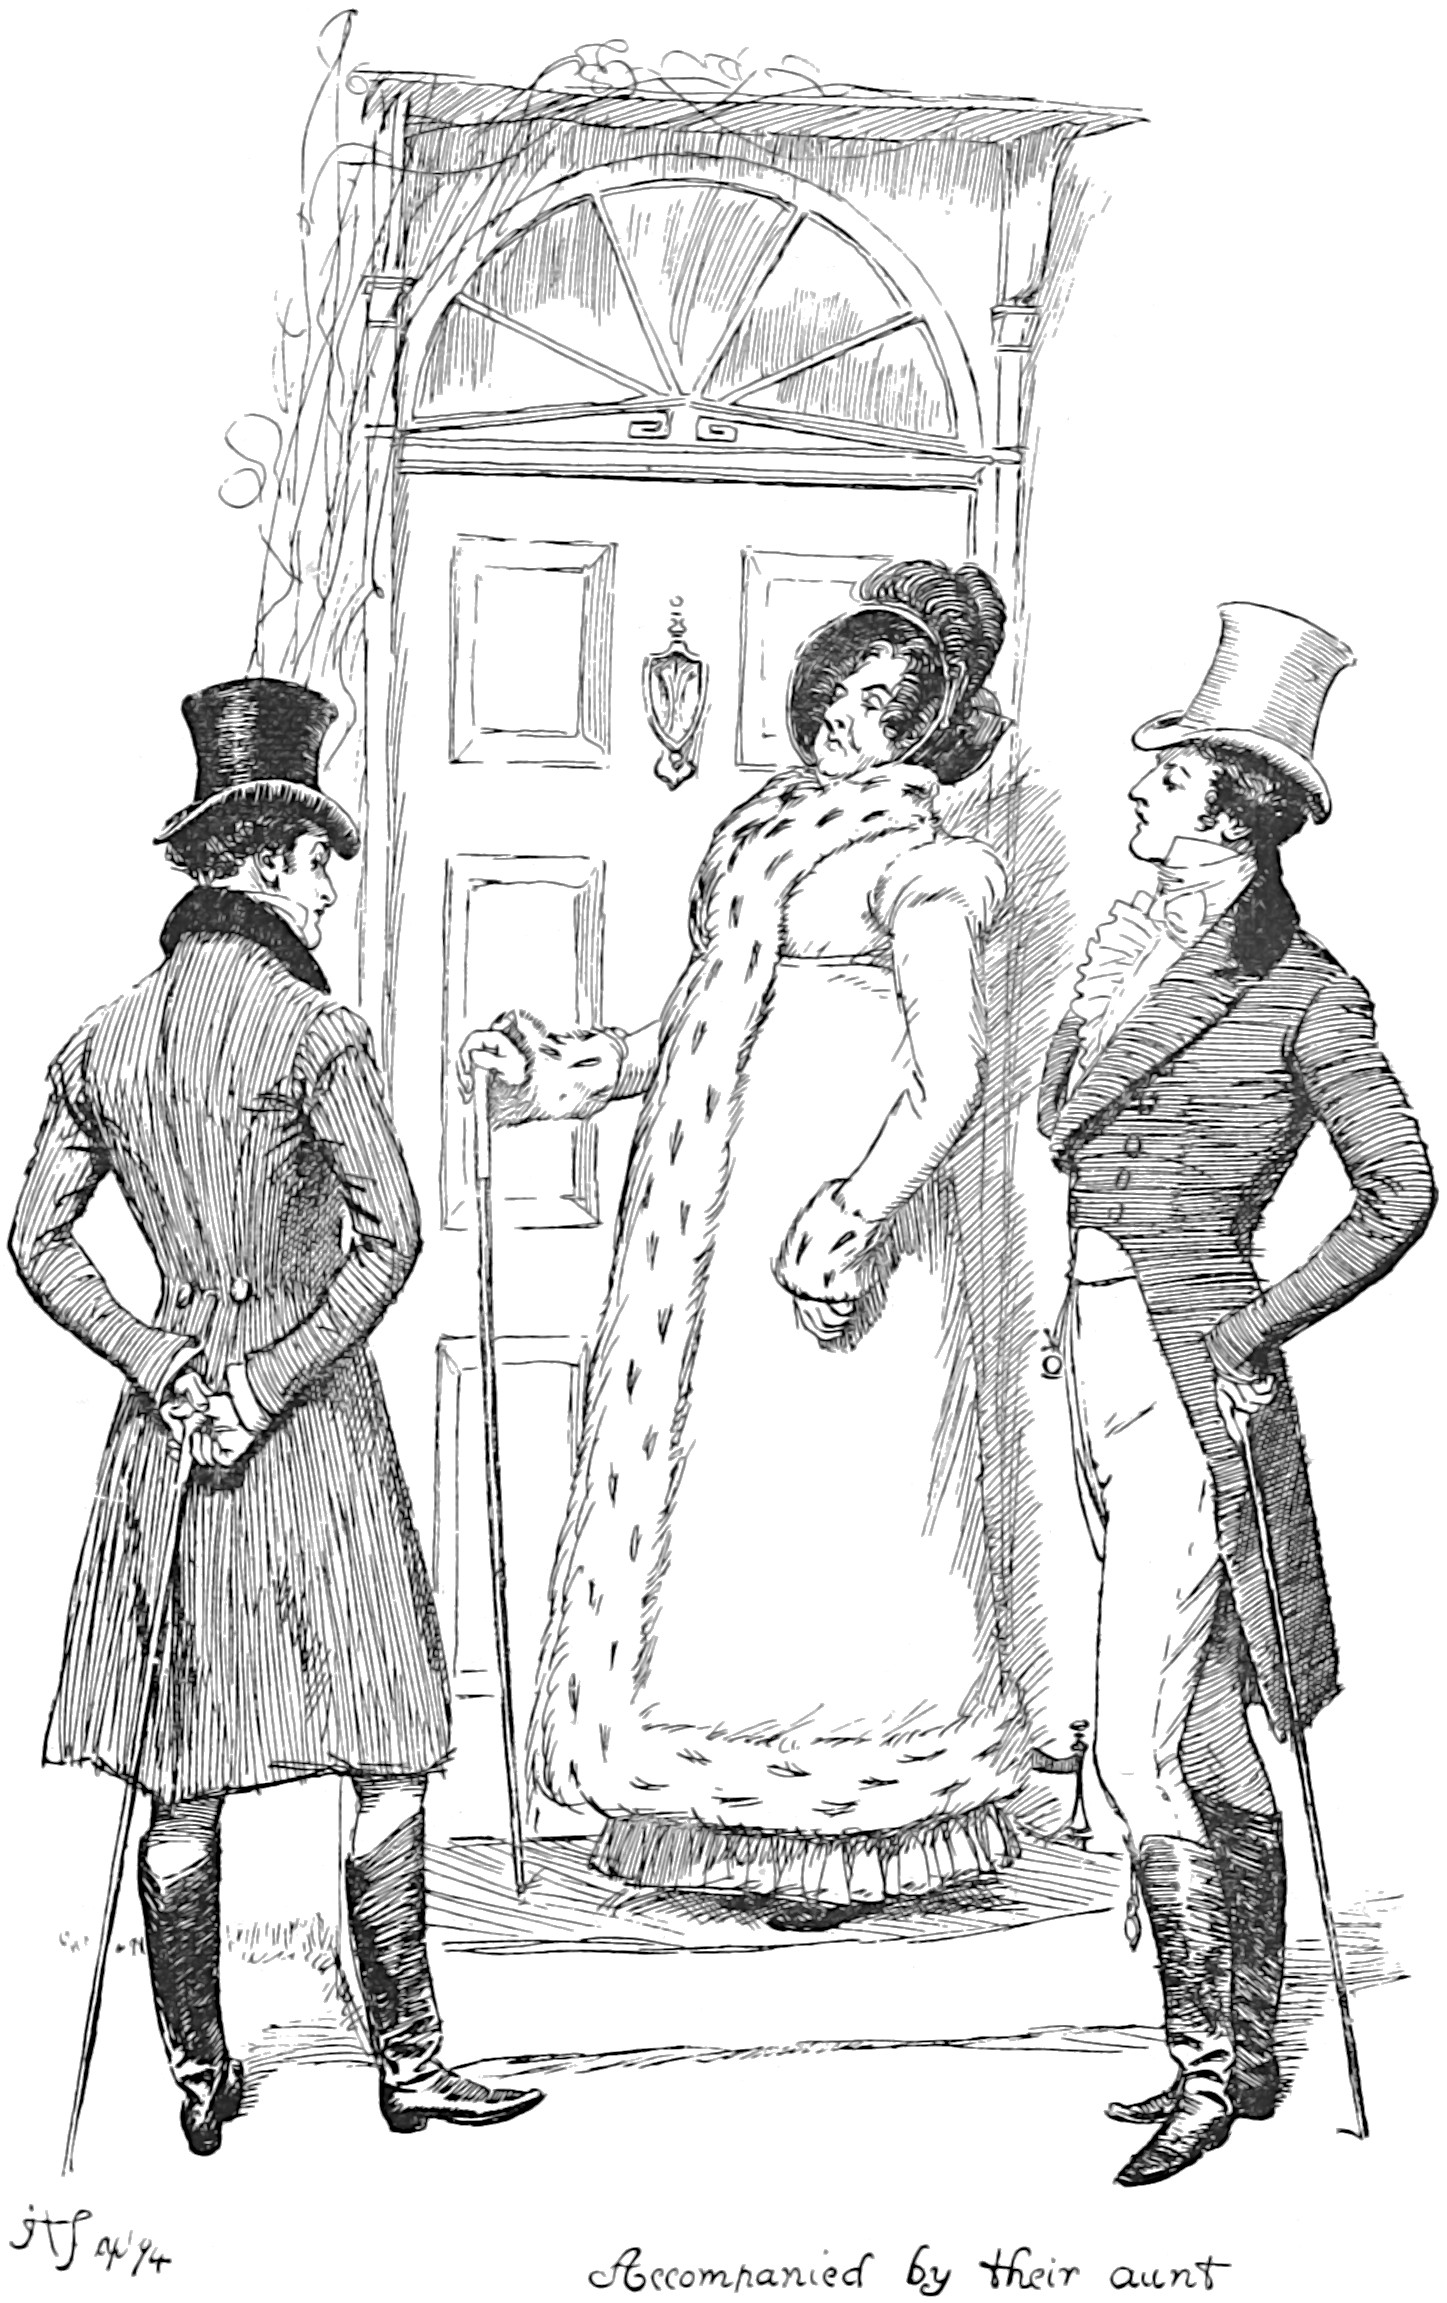
\includegraphics[width=\linewidth]{32aunt}
\captionlistentry{Accompanied by their aunt}
\end{figure}

Mr Darcy drew his chair a little towards her, and said, »\textit{You} cannot have a right to such very strong local attachment. \textit{You} cannot have been always at Longbourn.«

Elizabeth looked surprised. The gentleman experienced some change of feeling; he drew back his chair, took a newspaper from the table, and, glancing over it, said, in a colder voice,—

»Are you pleased with Kent?«

A short dialogue on the subject of the country ensued, on either side calm and concise—and soon put an end to by the entrance of Charlotte and her sister, just returned from their walk. The \textit{tête-à-tête} surprised them. Mr Darcy related the mistake which had occasioned his intruding on Miss Bennet, and, after sitting a few minutes longer, without saying much to anybody, went away.

»What can be the meaning of this?« said Charlotte, as soon as he was gone. »My dear Eliza, he must be in love with you, or he would never have called on us in this familiar way.«

But when Elizabeth told of his silence, it did not seem very likely, even to Charlotte's wishes, to be the case; and, after various conjectures, they could at last only suppose his visit to proceed from the difficulty of finding anything to do, which was the more probable from the time of year. All field sports were over. Within doors there was Lady Catherine, books, and a billiard table, but gentlemen cannot be always within doors; and in the nearness of the Parsonage, or the pleasantness of the walk to it, or of the people who lived in it, the two cousins found a temptation from this period of walking thither almost every day. They called at various times of the morning, sometimes separately, sometimes together, and now and then accompanied by their aunt. It was plain to them all that Colonel Fitzwilliam came because he had pleasure in their society, a persuasion which of course recommended him still more; and Elizabeth was reminded by her own satisfaction in being with him, as well as by his evident admiration, of her former favourite, George Wickham; and though, in comparing them, she saw there was less captivating softness in Colonel Fitzwilliam's manners, she believed he might have the best informed mind.




But why Mr Darcy came so often to the Parsonage it was more difficult to understand. It could not be for society, as he frequently sat there ten minutes together without opening his lips; and when he did speak, it seemed the effect of necessity rather than of choice—a sacrifice to propriety, not a pleasure to himself. He seldom appeared really animated. Mrs Collins knew not what to make of him. Colonel Fitzwilliam's occasionally laughing at his stupidity proved that he was generally different, which her own knowledge of him could not have told her; and as she would have liked to believe this change the effect of love, and the object of that love her friend Eliza, she set herself seriously to work to find it out: she watched him whenever they were at Rosings, and whenever he came to Hunsford; but without much success. He certainly looked at her friend a great deal, but the expression of that look was disputable. It was an earnest, steadfast gaze, but she often doubted whether there were much admiration in it, and sometimes it seemed nothing but absence of mind.

She had once or twice suggested to Elizabeth the possibility of his being partial to her, but Elizabeth always laughed at the idea; and Mrs Collins did not think it right to press the subject, from the danger of raising expectations which might only end in disappointment; for in her opinion it admitted not of a doubt, that all her friend's dislike would vanish, if she could suppose him to be in her power.

In her kind schemes for Elizabeth, she sometimes planned her marrying Colonel Fitzwilliam. He was, beyond comparison, the pleasantest man: he certainly admired her, and his situation in life was most eligible; but, to counterbalance these advantages, Mr Darcy had considerable patronage in the church, and his cousin could have none at all.